\documentclass{article}
\usepackage{arxiv}
\usepackage[T1]{fontenc}
\usepackage[utf8]{inputenc}
\usepackage{amsmath,amssymb}
\usepackage{booktabs,tabularx,array}
\usepackage[numbers,sort&compress]{natbib}
\usepackage{microtype}
\usepackage{xcolor}
\usepackage{graphicx}
\usepackage{pgfplots}
\pgfplotsset{compat=1.18}
\usepackage{url}
\usepackage[colorlinks=true,linkcolor=black,citecolor=black,urlcolor=blue!45!black]{hyperref}
\hypersetup{pdftitle={Description Logic Programs Revisited: The Benefits and Limits of Specialized Ontology Reasoning},pdfauthor={Raphael Volz}}
\renewcommand{\shorttitle}{Description Logic Programs Revisited}
\renewcommand{\headeright}{Raphael Volz}
\renewcommand{\undertitle}{Preprint}
\newcolumntype{Y}{>{\raggedright\arraybackslash}X}
\title{Description Logic Programs Revisited:\\The Benefits and Limits of Specialized Ontology Reasoning}
\author{Raphael Volz\\Pforzheim University}
\date{9 September 2026}

\begin{document}
\maketitle
\begin{abstract}
Restricting the expressive power of a knowledge representation language can
make reasoning more efficient, but the conditions under which this advantage
appears require empirical examination. We revisit Description Logic Programs,
which connect ontology languages with rule-based inference, through a
reconstruction of the original work and experiments on changing knowledge and
query answering. We investigate whether sharing explanations and adapting the
order of reasoning reduce computation while preserving its conclusions.
Sharing explanations accelerates a favourable update task by approximately
7.5 times, with a similar result in a separate replication, but adds 18--19\%
overhead when suitable explanations are absent. Adaptive evaluation reduces
some intermediate work without consistently improving complete task times.
Comparisons with established reasoners likewise reveal operation-specific
advantages and substantial disadvantages. The original Bach examples also
exposed a loss of valid conclusions during deletion in the tested ZodiacEdge
rule reasoner. On a finite task involving the
existence of unnamed individuals, specialized reasoning is 2.6--21.5 times
faster than the tested HermiT distribution; the task also belongs to the
established OWL 2 EL profile. These findings support a conditional account of
specialization: benefits depend on the structure of the knowledge, the change,
and the question. A fragment's theoretical or computational value is distinct
from how frequently it is used. The evidence supports useful specializations,
without establishing a general performance advantage or a new complexity bound.
\end{abstract}
\keywords{Ontology reasoning \and Description Logic Programs \and knowledge representation
\and incremental reasoning \and experimental evaluation}

\section{Introduction}
A knowledge base contains more than a collection of observations. Statements
about categories and relationships allow further conclusions to be drawn.
In the thesis's Bach family example, Johann Ambrosius can be identified as a
father even though the description does not name his child. An ontology
reasoner makes such implications explicit.
The challenge is to provide useful expressive power while keeping inference
manageable, especially when the observations or the governing statements
change.

Description Logic Programs (DLP) address this challenge by connecting a
restricted ontology language with rule-based inference~\cite{grosof2003}.
The 2004 thesis \emph{Web Ontology Reasoning with Logic Databases} developed
this connection into reasoning services and methods for maintaining inferred
knowledge~\cite{volz2004,volz2003maintenance}. Over the following two decades,
research advanced the treatment of alternative explanations, shared
computation, and the order of inference. Standardized OWL 2 profiles also
established several language restrictions intended for different reasoning
needs~\cite{owlprofiles2012}.

These developments raise a scientific question that is broader than whether
an old implementation can be made faster: under what conditions does
specialization remain useful? A restricted language can offer a mathematical
advantage even when its practical prevalence is unknown. A particular reasoner
can also outperform a broader one on a defined task without demonstrating a
new mathematical separation. Neither kind of evidence alone establishes that
the historical language interface is the best choice for all applications.

We examine three questions. First, when can explanations shared across many
individuals reduce the cost of keeping conclusions up to date? Second, when
does avoiding intermediate reasoning work reduce the time required for a
complete task? Third, can reasoning within an expressive DLP fragment offer
computational value relative to a broader OWL reasoner, independently of how
often applications use that fragment alone?

The study combines semantic reconstruction, controlled experiments, and
comparisons with external reasoners. It includes deliberately unfavourable
cases and reports unsuccessful interventions. The research questions organize
an exploratory programme developed in stages; they are not presented as a
retrospectively preregistered experiment. A focused review of the original
specification establishes the meaning the reconstruction must preserve.
Constructed workloads then isolate proposed mechanisms, while established
university and database workloads test selected tasks beyond those examples.

The contribution is an empirical reassessment of DLP and an account of the
conditions under which the examined specializations help or fail. The original
connection between ontology languages and rules, support-aware maintenance,
and adaptive query evaluation remain attributable to earlier work. The new
evidence concerns the tested combination of shared explanations, bounded
adaptation, and matched reasoning tasks. It provides preservation arguments
and evidence against unconditional performance expectations, rather than claiming
a generally superior reasoning algorithm.

\section{Background and related research}
\label{sec:background}

An ontology describes categories, relationships, and constraints within a
domain. An ontology reasoner determines what follows from these descriptions
and the available observations. We use the thesis's original Bach family
knowledge base as a running illustration~\cite[Table~2.5, p.~35]{volz2004}.
It describes Johann Ambrosius as a man with a male child, without naming that
child. It also states that men are persons and defines a father as a man with
a child who is a person. A reasoner can therefore conclude that Johann
Ambrosius is a father without identifying his child. This distinguishes an
implied conclusion from an explicitly recorded statement.

Missing information is also different from falsehood. The same knowledge base
names Wilhelm Friedemann as Johann Sebastian's child. As the thesis explains,
this does not establish that he is Johann Sebastian's only child
\cite[Example~5.4.1, p.~131]{volz2004}. Incomplete family records do not rule
out additional children.

A complementary illustration comes from the Lehigh University Benchmark
(LUBM), used in our external comparisons~\cite{guo2005,lubmwebsite}.
Its ontology states that every graduate student is a person who takes some
graduate course, that graduate courses are courses, and that people taking
courses are students. A graduate-student declaration therefore implies
student membership even when it names no course. This distinction matters
for LUBM's sixth query, which asks for all students. Bach connects the present
study to the original work; LUBM connects the same reasoning ideas to an
established benchmark.

The Web Ontology Language, OWL, gives such statements a precise meaning
\cite{owl2004,owldirect2012}. Greater expressive power permits more complex
descriptions, but can make inference more demanding. A central research
question is therefore which restrictions preserve useful forms of expression
while enabling simpler reasoning. A \emph{fragment} is a language obtained by
such restrictions. Its value can arise from a mathematical guarantee, a
computational advantage on a specified task, or both.

Description Logic Programs were introduced as a connection between ontology
languages and rules of the form ``if these conditions hold, then this
conclusion follows''~\cite{grosof2003}. Volz's 2004 thesis developed this
connection into methods for answering questions and maintaining inferred
knowledge as facts and rules change~\cite{volz2004}. The original research
already addressed changes to the ontology's rules, rather than only changes
to observations~\cite{volz2003maintenance}. The work examined here inherits
that problem and semantic foundation. Its expressive mode, called DLP L3,
also admits statements requiring an individual to exist without naming them.
The thesis illustrates this using Johann Ambrosius's unnamed child
\cite[Example~4.5.2, p.~94]{volz2004}. This additional capability requires separate
attention to whether a reasoning procedure terminates.

One influential approach computes consequences in advance and retains them
for later questions. This is called \emph{materialization}. Its main attraction
is that repeated questions can reuse earlier deductions. Its main difficulty
is maintaining those deductions when their premises change. Adding a new
premise usually creates further conclusions. Removing one is subtler: a
conclusion may have several independent justifications. The thesis's extended
Bach family tree supplies two paths from Johannes to Wilhelm Friedemann, one
through Johann Sebastian and another through Maria Barbara. In its hypothetical
withdrawal of the Johann Sebastian--Wilhelm Friedemann link, Johannes remains
an inferred ancestor through Maria Barbara
\cite[Section~6.2.1 and Figure~6.2, p.~150]{volz2004}. The example changes the
recorded knowledge, rather than making a historical claim about parentage.

Research has developed this idea in several directions. Deletion and
rederivation, established before the thesis, first withdraw potentially affected
conclusions and then restore those still justified~\cite{gupta1993}.
Subsequent methods examine alternative proofs more selectively, count suitable
forms of support, or combine specialized procedures
\cite{motik2015bf,hu2018,motik2019,hu2022modular}. Changes to the rules
themselves have also received renewed attention
\cite{kotowski2011,xu2023}. These studies establish the broader principle
that maintenance should depend on the structure of the affected reasoning,
not simply on the number of changed statements.

A second direction reduces repeated work across similar deductions.
Type-based reasoning groups individuals with recurring descriptions, while
compressed reasoning represents repeated patterns more economically
\cite{bajraktari2017,hu2019compressed}. Parallel and column-oriented
systems organize computation and storage to handle larger knowledge bases
\cite{motik2014parallel,carral2019}. More recent work further specializes
representations for common patterns~\cite{zhang2024}. These approaches
motivate our investigation of whether individuals with the same current
starting facts can share the work of establishing a surviving justification.
The general idea of sharing proofs is inherited; the present study tests a
restricted form of it during simultaneous changes to facts and rules.

A third direction concerns the order in which conditions are tested. Combining
records that satisfy several conditions is known as a \emph{join}. An
unfavourable order can produce many temporary combinations that later tests
discard. Research has established stronger algorithms for combining multiple
relations~\cite{ngo2012}, and recent studies investigate robust filtering
and the avoidance of unnecessary intermediate expansion
\cite{qiao2026,bekkers2025}. These findings motivate our experiments with
limited adaptation of evaluation order. Their mathematical guarantees do not
automatically apply to the simpler strategy examined here.

Finally, OWL 2 profiles formalize different restrictions for different
reasoning needs. The rule-oriented RL profile explicitly acknowledges DLP
among its influences~\cite{owlprofiles2012}. This historical continuity
motivates reassessment rather than a claim that the earlier fragments have
become obsolete. Our contribution is a corrected reconstruction and a
controlled investigation of when selected restrictions and reasoning
strategies help, including cases in which their costs outweigh their benefits.

\section{Study design}
\label{sec:methods}
The study developed in stages. We first examined two ways of reducing repeated
reasoning after changes to a knowledge base, then used the observed costs and
the literature review to select further experiments. The later questions and
comparisons were therefore exploratory. Protocols were recorded before their
respective timing series, but the research programme was not publicly
preregistered. Earlier trials, unsuccessful cases, and subsequent replications
are retained in the supplementary evidence.

\subsection{Interventions and comparisons}
The first intervention changes how groups of records satisfying a rule's
conditions are combined. One option first collects the records affected by a
change; another starts with records meeting all the conditions and then checks
which were affected. We investigated whether information about recent changes
helps choose between these equivalent approaches, including the cost of the choice.

The second intervention shares explanations for conclusions that remain valid
after a change. Several individuals may satisfy exactly the same relevant
conditions. When they do, one calculation can establish which conclusions
still follow for all of them. These explanations can prevent unnecessary
withdrawal and restoration of conclusions. If no suitable explanation is
found, the ordinary maintenance procedure still determines the answer. This
restricted use of shared explanations builds on support-aware maintenance and
shared reasoning~\cite{motik2015bf,hu2018,hu2019compressed,hu2022modular}.

Follow-up changes reduced repeated work in three further ways: reusing checks
that remain valid when information is added, updating access structures only
where information has changed, and preparing common rule operations for
repeated use. These changes apply established techniques; the experiment
evaluates their combined effect. A later experiment reconsidered evaluation
order by briefly examining likely consequences of alternative choices. This
was motivated by recent work on avoiding large intermediate results
\cite{qiao2026,bekkers2025}. The examination changes the search order, without
excluding possible answers.

We distinguish three comparisons. Controlled variants of the same system
estimate an intervention's effect. Comparisons with a preserved earlier
version describe cumulative progress. Executing an independent reasoner on
matched inputs and tasks tests relative performance beyond the local system.
Published timings on different machines provide context, but cannot supply
speed ratios for our experiments.

\subsection{Controlled and established workloads}
The initial experiment combined the first two interventions in a factorial
design: each was either present or absent, yielding four variants. Eighteen
constructed cases varied the concentration of changes, surviving explanations,
recursion, and opportunities to share reasoning. Nine repetition blocks tested
all variants in fresh processes, with a rotating order. Complete update time
was the primary outcome. A separate replication used new random seeds and
144 fresh processes to re-examine the main explanation-sharing benefit and its
adverse cases. It supplements the original observations rather than replacing
them.

External validation began with LUBM, which
provides a university ontology, generated data, and reference answers
\cite{guo2005,lubmwebsite}. We used one generated university and retained the
logical ontology. Three repetition blocks compared three local variants, and
all fourteen queries were checked against the complete official answer sets.
This tests established questions on a modest dataset; it is not a scalability
study.

For changing rules, we used the positive university rule programme supplied
with ZodiacEdge~\cite{xu2023,zodiacartifact}. Two scenarios added and removed
designated sets of eight and sixteen rules. Four repetition blocks compared
four local variants; a separate four-block comparison alternated our candidate
and ZodiacEdge itself. Additional samples removed and restored 1,000 facts,
following the update size used in earlier maintenance research~\cite{hu2018}.
Samples within one process are repeated observations, not independent process
replicates. The author's rule programme and the complete LUBM ontology are
distinct reasoning tasks.

The Transaction Processing Performance Council's Benchmark H (TPC-H) evaluates
database systems answering analytical questions over business data~\cite{tpch}.
Our query experiments used the conditions underlying its queries Q3, Q5,
and Q9 at two data scales. These six components retain the combinations of
input rows satisfying each query, but exclude aggregation and result ordering.
They therefore do not constitute a full TPC-H evaluation or reproduce the
larger study of Qiao and colleagues~\cite{qiao2026}. The first comparison used
three blocks, with all three components evaluated sequentially in each fresh
process. A follow-up gave each component its own process and compared three
variants across three blocks. It added controls deliberately chosen to expose
unhelpful decision costs and misleading intermediate patterns, giving 90
processes overall. The follow-up revisits the workload that motivated it;
it does not provide independent evidence of generalization.

\subsection{Expressiveness, correctness, and measurement}
A separate experiment compared our reasoner with HermiT~\cite{glimm2014hermit}
on a finite family using existential statements: every member of one class
must relate to some member of another. Both systems determined consistency
and returned all named members of two target classes. Populations of 100,
1,000, and 10,000 individuals were tested in three blocks, comparing the
candidate, its earlier baseline, and HermiT. These 27 processes test a selected
DLP L3 task beyond the structural OWL 2 RL syntax. The family also belongs to
OWL 2 EL~\cite{owlprofiles2012}, and its answers do not require explicitly
constructing the unnamed individuals. It tests computational specialization,
without assuming that such ontologies are common.

Correctness was checked separately from performance. Update experiments
compared complete conclusions with fresh recomputation; small cases also used
independently written reference procedures. Query experiments checked exact
answers against official LUBM answers or independent database evaluation.
The existential experiment used independently justified answers and controls
omitting each essential statement. Agreement of counts alone was insufficient.

A further comparison returned to the original Bach examples at their original
scale~\cite[Table~2.5, p.~35; Figure~6.2, p.~150]{volz2004}. The current
reasoner, its preserved earlier version, and HermiT answered 25 questions on
the complete ontology. A separate family task asked nine questions, including
the complete ancestor and dynasty relationships. All four systems evaluated
the original and three changed family states from scratch; the two local
versions and ZodiacEdge also applied and reversed each change while retaining
state. Twelve repetition blocks specified 336 fresh processes, with rotating
system order. The older version was measured anew: its saved historical
results contained no Bach comparison. These small examples test source fidelity
and update behaviour, without making a scaling claim.

For this comparison, the complete ontology's existence requirements and
constraints fall outside ZodiacEdge's positive-rule task. Its family evaluation
uses the same recorded relationships and rules. A wrong answer disqualifies
the entire system--task combination from a timing ranking; passing executions
are not selected to hide unsuccessful ones. Separate diagnostic checks
investigate discrepancies while retaining the recorded implementation.

Timings include complete updates or complete consumption of query answers.
Query computation and data preparation are reported separately, with combined
costs where measured. HermiT comparisons include loading, consistency, and
answer retrieval because systems perform inference at different stages.
Independent checks lie outside these task intervals. In controlled comparisons,
ratios pair observations within repetition blocks and report their median,
rather than dividing two separately calculated medians. Historical comparisons
use ratios of the medians from separate runs.

All new measurements used one Apple M4 Max desktop. Process restarts did not clear
filesystem caches. Unrelated activity may have overlapped the primary study;
its extent is unknown, and the original samples were retained. Later timed
studies were scheduled separately. Small repetition counts, one host, and
selected workloads make the comparisons descriptive. Detailed protocols,
timing boundaries, individual observations, and preservation arguments are
provided in the supplement.


\section{Results}
\label{sec:results}
\subsection{A semantic basis for comparison}
The reconstruction exposed consequential inconsistencies in particular printed
formulas and procedures. For example, separate questions about the equivalence
of two categories can interfere if their test assumptions are combined and
individuals may denote the same object. Similarly, withdrawing a rule must
remove conclusions whose only explanation depends on that rule. The
supplement gives explicit counterexamples and the required corrections.
These findings concern the specification. The historical implementation was
not examined, so its behaviour cannot be inferred from these findings.

The experiments evaluate the corrected interpretation. The complete official
answer sets for all fourteen LUBM questions were recovered in every measured
run. The earlier controlled update experiments matched the full conclusions
of fresh recomputation, and the external query comparisons matched independently
established answers. The later Bach comparison also records an external
update discrepancy, discussed below.
These checks support the interpretation of the measured tasks. They do not
establish correctness for all possible ontologies or make the distinct
benchmark tasks semantically interchangeable.
Table~\ref{tab:scientific-evidence} summarizes the principal comparisons and
their different evidential roles.

\subsection{Sharing explanations helps when explanations survive}
In the favourable constructed case, many individuals shared starting facts
and retained an independent reason for a conclusion after a change. Establishing
that reason once avoided withdrawing and rebuilding the same kind of
conclusion repeatedly. The median of paired update-time ratios was approximately
0.134, corresponding to a 7.45-fold improvement. A separate replication
obtained a 7.56-fold improvement on the corresponding case.

When no suitable explanation survived, the search for one could not prevent
the required removals. It nevertheless consumed time, producing approximately
18--19\% overhead. The replication reproduced both the benefit and this cost.
Cases with less opportunity to share explanations gave more limited benefits.
Figure~\ref{fig:scientific-support} shows the full range of the replication's
cases, including the adverse outcomes.

The result supports a mechanism with identifiable conditions. Reuse is
valuable when the same valid reasoning applies to many individuals and avoids
a substantial amount of repeated work. Attempted reuse can be harmful when
those conditions are absent. The experiments therefore support conditional
use, not an expectation that additional explanation checking always improves
maintenance.

% Generated from preserved paired observations. Do not edit by hand.
\begin{figure}[htbp]
\centering
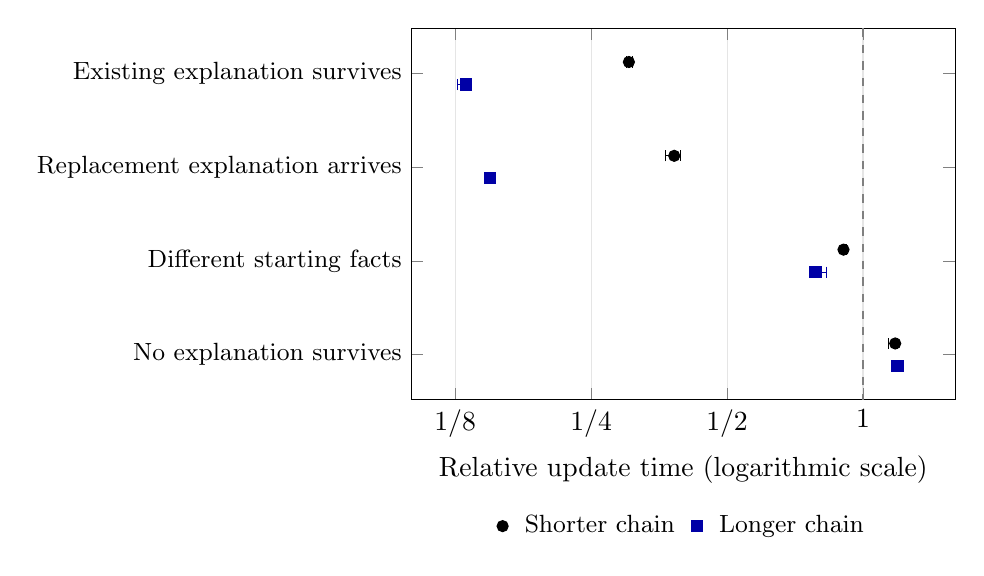
\begin{tikzpicture}
\begin{axis}[width=0.70\linewidth,height=6.3cm,xmode=log,
xmin=0.1,xmax=1.6,ymin=-0.48,ymax=3.48,y dir=reverse,
ytick={0,1,2,3},
yticklabels={{Existing explanation survives},{Replacement explanation arrives},{Different starting facts},{No explanation survives}},
yticklabel style={font=\small},
xlabel={Relative update time (logarithmic scale)},
xtick={0.125,0.25,0.5,1},xticklabels={1/8,1/4,1/2,1},
xmajorgrids=true,grid style={gray!20},
legend style={at={(0.5,-0.28)},anchor=north,draw=none,font=\small,column sep=4pt},
legend columns=2]
\addplot[gray,dashed,forget plot] coordinates {(1,-0.48) (1,3.48)};
\addplot[only marks,mark=*,black,error bars/.cd,x dir=both,x explicit]
coordinates {
(0.303107186,-0.12) += (0.005380192,0) -= (0.003875500,0)
(0.381928514,0.88) += (0.012880738,0) -= (0.016163149,0)
(0.905277511,1.88) += (0.011728574,0) -= (0.005298335,0)
(1.178358201,2.88) += (0.016322907,0) -= (0.041958422,0)
};
\addlegendentry{Shorter chain}
\addplot[only marks,mark=square*,blue!65!black,error bars/.cd,x dir=both,x explicit]
coordinates {
(0.132315292,0.12) += (0.001499708,0) -= (0.005665689,0)
(0.149473165,1.12) += (0.003692939,0) -= (0.001777688,0)
(0.784898536,2.12) += (0.047034643,0) -= (0.012522867,0)
(1.187932124,3.12) += (0.040023678,0) -= (0.034218154,0)
};
\addlegendentry{Longer chain}
\end{axis}
\end{tikzpicture}
\caption{Sharing explanations reduces the cost of updating knowledge when conclusions remain justified, but adds work when their justification disappears. The experiment changes facts and rules in cyclic chains concerning 256 individuals; the shorter and longer chains have four and 32 links before the cycle closes. Points show median time with shared explanations divided by ordinary maintenance time, from nine paired repetitions per case in an independent replication. Bars show descriptive 95\% paired bootstrap intervals (2,000 resamples). Values left of the dashed line indicate faster updating.}
\label{fig:scientific-support}
\end{figure}

\begin{table}[htbp]
\centering\small
\caption{The principal comparisons answer different scientific questions; they do not establish an overall ranking of reasoning systems. Performance changes are derived from median paired time ratios on the same machine. Query timings in the fourth row exclude data preparation.}
\label{tab:scientific-evidence}
\begin{tabularx}{\linewidth}{@{}>{\raggedright\arraybackslash}p{0.19\linewidth}>{\raggedright\arraybackslash}X>{\raggedright\arraybackslash}X@{}}
\toprule
Evidence & Comparison & Principal finding \\
\midrule
University ontology & Full LUBM ontology and its 14 standard questions. & All reference answers recovered in every repetition. \\[4pt]
Changes to rules & Established university rule program, compared with the reference version. & Rule additions 2.1--3.2\,$\times$ faster; removals 1.4--1.6\,$\times$ faster. \\[4pt]
External rule reasoner & The same rule changes, compared with ZodiacEdge. & One addition 6.2\,$\times$ faster; one removal 41\,$\times$ slower. \\[4pt]
Order of reasoning & A difficult TPC-H Q5 component and four deliberately adverse controls. & Q5 needs 49\% less query time; controls need 7--24\% more. \\[4pt]
Broader OWL reasoner & Selected DLP L3 task, compared with HermiT at three data sizes. & 2.6--21.5\,$\times$ faster; the tested family also belongs to OWL 2 EL. \\[4pt]
\bottomrule
\end{tabularx}
\end{table}


\subsection{Less intermediate work does not guarantee a faster task}
The first adaptive intervention changed how the sets satisfying a rule's
conditions were combined. In one case it avoided tens of thousands of
intermediate visits. Across the ten cases, however, the geometric mean of
paired complete-update ratios was 1.0014: there was no overall improvement.
Every reported uncertainty interval included one. Much of the task's cost
lay outside the condition evaluation that the intervention changed. The study
therefore does not establish a complete-task advantage from that reduction
in intermediate work.

The subsequent query experiment examined a different source of repeated work:
the order in which records satisfying several conditions were combined. On the
larger TPC-H Q5 component, a brief look ahead reduced examined candidates from
621,901 to 155,969. The median paired query-computation ratio was 0.510, with
an observed range of 0.481--0.520 across three repetitions. The computation
itself was therefore approximately twice as fast in this case.

The benefit did not extend uniformly to the complete task. Its paired
preparation-plus-query ratios ranged from 0.972 to 1.273, spanning both
improvement and deterioration. Variation in preparation costs preceded query
execution and cannot be attributed to the ordering decision on this evidence.
The four adverse controls became 6.6--23.8\% slower in query computation.
They retained the same number of examined candidates, exposing the cost of
making decisions that did not reduce subsequent work. The other five database
components showed no comparable reduction in candidates.

Together, the two experiments distinguish an algorithm's local opportunity
from the benefit of using it. Avoided combinations are a plausible mechanism,
but total cost also includes deciding what to do and preparing the data.
A promising reduction in one part of a task is insufficient evidence for a
general speed advantage.

\subsection{External comparisons reveal different strengths}
The new system reduced the two designated rule-insertion times by factors of
3.18 and 2.08 relative to the preserved local reference version. This establishes
progress against that reference, but an external comparison asks a different
question. On the same university rule program, it was approximately 6.2 times
faster than ZodiacEdge when inserting the eight-rule set. ZodiacEdge was
faster on several other operations, including deletion of the sixteen-rule set,
where our candidate took approximately 41 times as long. The corresponding
median deletion times were 0.97 seconds for our candidate and 0.023 seconds
for ZodiacEdge; the large relative difference concerns an operation taking
less than a second in either system at this scale.

All conclusions agreed for these university rule changes. The difference is therefore a performance
limitation on a matched task, not a trade of completeness for speed. A separate
diagnostic examination found that repeated preparation and checking dominated
the candidate's cost in that deletion case. The number of withdrawn
conclusions was exactly the number that should disappear. This observation
identifies a direction for further investigation, but does not demonstrate
how much of the external performance gap a future change would remove.

The final regression evaluation also preserved the less favourable local
outcomes. All 54 workloads passed their correctness checks. Although all 51
comparable initial-inference medians were lower than the saved reference in
that run, two of 36 update comparisons were slower, by 25.8\% and 2.7\%.
Those historical runs were not interleaved experiments and cannot isolate the
effect of the latest intervention. Neither local progress nor a selected
external win establishes an overall ranking.

\subsection{The original examples test preservation of meaning}
The Bach comparison returns to the examples that motivated the reconstruction.
It covers the complete ontology's 25 questions and nine questions on the
separate family graph, including all ancestor and dynasty relationships.
These original examples are small: their timings describe the cost of answering
and maintaining a particular set of questions, rather than performance on
large family histories.

The full Bach ontology gave identical answers to all 25 questions in the three supported systems. Median complete-task time was 55.6 ms for the current reasoner, 89.5 ms for the preserved earlier implementation, and 347.4 ms for HermiT.

All four systems agreed on the complete family answers when each resulting state was computed from scratch. During incremental fact replacement, however, the pinned ZodiacEdge implementation failed exact-answer validation in every second (6/12) process. This task therefore receives no ZodiacEdge timing ranking. The current and earlier implementations passed every tested update and restoration. Detailed phase and process times are given in the supplement.

ZodiacEdge had lower task times on all four family reconstructions and both rule changes. For the original family, its median task time was 4.4 ms, compared with 7.5 ms for the current reasoner. Including process startup, checking and shutdown, the corresponding medians were 137.9 and 135.6 ms. The timing boundary therefore matters on these small inputs.


Independent checks of the recorded ZodiacEdge version exposed a limitation in
one family update. After withdrawing the Johann Sebastian--Wilhelm Friedemann
link and inserting another, some executions lost the conclusion that Johannes
is an ancestor of Wilhelm Friedemann. The path through Maria Barbara still
justifies that conclusion. Recomputing the changed family from its assertions
provides a separate check of the required result. The discrepancy concerns
the tested incremental operation in that version; it does not contradict the
successful checks on the earlier university rule changes.

The affected system--task combination is excluded from performance rankings.
Retaining this discrepancy is part of the comparison: an apparently quicker
operation cannot count as an improvement when it loses a required answer.
The evidence also distinguishes computing a changed state afresh from
maintaining it through a sequence of changes.

\subsection{A restricted language can offer computational value}
The existential reasoning experiment examines the distinction between existence
and naming illustrated by Johann Ambrosius's unnamed child and LUBM's unnamed
course. It uses a separate, simplified family of constructed ontologies:
belonging to one class requires a
related individual to exist, and that relationship implies membership in
another class. These measured inputs are distinct from both illustrative
ontologies. The
existential statement is essential to the tested conclusion; removing it
changes the correct answer. Its form goes beyond the permitted syntax of
OWL 2 RL.

Across the three populations, the candidate's paired task-time ratios to
HermiT were approximately 0.046, 0.263, and 0.378. These correspond to
21.5-, 3.8-, and 2.6-fold advantages for the selected tasks. At the largest
population, median task times were 0.94 seconds for the candidate and
2.48 seconds for HermiT. The result persists
when the entire fresh process is timed, including startup and completion:
the corresponding ratios are approximately 0.379, 0.476, and 0.415.
All systems agreed on consistency and the named individuals satisfying both
questions. Most of the advantage was already present in the earlier local
version, so it cannot be attributed to the latest optimizations.

This provides an example of useful computational specialization. It requires
no assumption about how commonly the fragment occurs. Its scope is nonetheless
specific: the family also belongs to OWL 2 EL, and the relevant conclusion can
be reached without explicitly constructing the unnamed individuals. The
experiment does not establish superiority over specialized EL reasoners or
performance on arbitrary existential ontologies.

\section{Discussion}
\label{sec:discussion}

The findings support a conditional account of efficient ontology reasoning.
Restricting a language can create opportunities for simpler computation, but
the benefit also depends on the arrangement of facts, the available
justifications, and the questions being asked. In the present experiments,
sharing surviving justifications was valuable when many individuals could
reuse the same reasoning. It became a cost when the attempted justification
did not exist. Similarly, spending more effort choosing an evaluation order
helped one demanding query, but imposed overhead on adverse cases. These
results identify conditions for improvement rather than a universally
preferable strategy.

The external comparisons make this distinction especially important. One
rule insertion was approximately six times faster than ZodiacEdge, whereas
one rule deletion was approximately forty-one times slower. Neither result
alone characterizes the relative quality of the two approaches. Together,
they show why an average across unlike operations can conceal a substantial
weakness. They also motivate a more discriminating question: which observable
properties of a change predict whether shared reasoning, selective
reconsideration, or broader recomputation will be most effective? The current
evidence does not yet establish a reliable general answer.

The Bach update discrepancy adds a distinct qualification. Successful
recomputation of a state does not establish that every path of changes leading
to it will preserve the same conclusions. The surviving family connection
supplies a small, independently understandable test of this requirement.
An observed failure in one recorded version warrants a reproducible
counterexample and a scoped conclusion, rather than a general ranking of
reasoning methods.

\subsection{The continuing value of restricted languages}

A fragment's scientific value does not depend on knowing how frequently it
is used in practice. A proven reduction in computational difficulty is
valuable even without an adoption survey. Prior work on description logics
whose statements take a restricted implication form, known as Horn description
logics, illustrates this point: restricting the form of logical statements
changes the established complexity of specified reasoning tasks
\cite{hustadt2005}. That result concerns precisely defined languages and
tasks. It does not, by itself, supply a complexity guarantee for the DLP L3
fragment or the reasoning procedure studied here.

Measured performance provides a different kind of evidence. On the earlier
constructed existential family, the specialized reasoner checked consistency and identified the
individuals satisfying the same questions faster than HermiT, which supports a broader OWL
language~\cite{glimm2014hermit}. This demonstrates a useful computational
specialization under the experimental conditions. It does not prove that all
DLP L3 tasks are easier, that the advantage grows indefinitely with input size,
or that restricting the language is the sole cause of the observed difference.
Much of the advantage was already present before the new optimizations.

That constructed family also belongs to OWL 2 EL, another established
restricted language. This qualification concerns the constructed experiment;
the full Bach ontology has a separate semantic scope. The result therefore leaves
open how the approach compares with reasoners specialized for EL. Moreover,
although the experimental statements require related individuals to exist,
a reasoner can derive the relevant class memberships without explicitly
constructing those individuals. The experiment establishes an advantage for the
specified questions; it does not establish an advantage of generating unnamed
individuals.

The relationship between the examined fragments and OWL 2 RL is one of
overlap, rather than a simple hierarchy. DLP L3 permits general statements
requiring the existence of a related individual, which lie outside RL's
permitted syntax. Conversely, RL includes constructs absent from the
reconstruction~\cite{owlprofiles2012}. It would therefore be misleading
to describe DLP L3 as a superset of RL or all the historical fragments as RL
subsets. Language membership, the meaning assigned to statements, and the
questions a procedure can answer completely must be assessed separately.

\subsection{Limits of the evidence and further questions}

The benchmark collection combines controlled examples, a university ontology,
the thesis's original Bach examples, changes to a published rule program,
and selected database query components.
This diversity tests several mechanisms, but does not constitute a
representative sample of ontology applications. The database components omit
parts of the full published workloads. Repeated measurements on one machine
provide local evidence, with limited information about variation across
hardware, systems, or larger datasets. Historical published timings provide
context, not directly comparable speed measurements.
The Bach examples retain their original small scale; repeating their
measurements does not turn them into a scalability study.

Agreement with independently justified answers strengthens confidence in the
reported experiments. It cannot establish correctness for every ontology,
nor certify the thesis's historical software. Likewise, corrections to
particular printed formulas and procedures do not invalidate the underlying
connection between ontology semantics and rule evaluation. They indicate
where the specification needs repair and where experimental reconstruction
can contribute to scientific scrutiny.

Further studies can test three propositions. First, the benefit of shared
justifications should increase with the proportion of individuals that share
both starting facts and surviving proofs. Second, selective rule-maintenance
methods should be most advantageous when a change affects a small part of
the reasoning dependencies. Third, choosing an evaluation order should help
only when avoided combinations compensate for the cost of making that choice.
Experiments that vary these properties independently would provide stronger
causal evidence than adding more undifferentiated benchmarks.

Broader comparisons should also include specialized EL reasoners and diverse
DLP L3 tasks, with explicit termination and completeness conditions. Some recursive
existential descriptions can make the present procedure generate an unending
sequence of unnamed individuals. Failure of this procedure to finish does not
establish that no other procedure could decide the same question. A separate
study could examine how often real ontologies and their application questions
fit each fragment. Such a survey would inform practical adoption, but its
difficulty does not postpone the theoretical or computational case for
studying restricted languages.


\section{Conclusion}
Description Logic Programs offer useful computational specializations, with
advantages that depend on the knowledge, the change, and the question.
Sharing valid explanations reduced selected update costs, while unsuccessful
searches added work. Changing evaluation order reduced some intermediate
results without consistently improving complete task times. The DLP L3
comparisons with HermiT demonstrate benefits on defined tasks, while the
mixed ZodiacEdge results show why performance must be assessed alongside
preservation of every required conclusion.

These findings support restricted reasoning languages without establishing
a general performance ranking or a new complexity bound. Their computational
value is distinct from their prevalence in applications. The next step is to
test whether observable properties of knowledge and updates predict the
reported benefits across broader, independently selected workloads.

\section*{Data, supporting material, and research transparency}
The technical supplement contains the semantic counterexamples, preservation
arguments, detailed protocols, full result tables, and reproducibility
information. The accompanying research artifact contains the code and saved
experimental observations; the
\href{https://github.com/volzinnovation/my-phd-thesis-gpt-6-astra}{project repository}
provides the development history.
The fixed reference results and earlier measurements are preserved.
The Bach comparisons add new observations of the thesis's original examples,
including fresh measurements of the preserved reference implementation.
AI assistance was used in implementation, literature retrieval, analysis, and
manuscript preparation. The manuscript has not been submitted to arXiv.

\setlength{\bibsep}{3pt}
\renewcommand{\bibfont}{\small\raggedright}
\bibliographystyle{plainnat}
\bibliography{references}
\end{document}
